  \chapter{Congruence Subgroups \& Modular Curves}
    Every holomorphic or Maass form is a special type of function depending on certain subgroups of $\PSL_{2}(\Z)$. These are the congruence subgroups. The associated modular curve is the quotient of the upper half-space $\H$ by an action of this subgroup. We introduce these topics first as they are the foundation for discussing holomorphic and Maass forms in complete generality.
    \section{Congruence Subgroups}
      The \textbf{modular group}\index{modular group} is $\PSL_{2}(\Z) = \SL_{2}(\Z)/\{\pm I\}$. That is, the modular group is the set of matrices with integer entries and of determinant $1$ determined up to sign. The reason we are only interested in these matrices up to sign is because the modular group has a natural action on the upper half-space $\H$ and this action will be invariant under a change in sign. The first result usually proved about the modular group is that it is generated by two matrices:

      \begin{proposition}\label{prop:PSL_generator}
          \[
            \PSL_{2}(\Z) = \left\<\begin{pmatrix} 0 &-1 \\ 1 & 0 \end{pmatrix},\begin{pmatrix} 1 & 1 \\ 0 & 1 \end{pmatrix} \right\>.
          \]
      \end{proposition}
      \begin{proof}
        Set $S$ and $T$ to be the first and second generators respectively. Clearly they belong to $\PSL_{2}(\Z)$. Also, $S$ and $T^{n}$ for $n \in \Z$ acts on $\g = \begin{psmallmatrix} a & b \\ c & d \end{psmallmatrix} \in \PSL_{2}(\Z)$ by
        \[
          S\g = S\begin{pmatrix} a & b \\ c & d \end{pmatrix} = \begin{pmatrix} -c & -d \\ a & b \end{pmatrix} \quad \text{and} \quad T^{n}\g = T^{n}\begin{pmatrix} a & b \\ c & d \end{pmatrix} = \begin{pmatrix} a+nc & b+nd \\ c & d \end{pmatrix}.
        \]
        In particular, $S$ interchanges the upper left and lower left entries of $\g$ up to sign and $T^{n}$ adds an $n$ multiple of the lower left entry to the upper left entry. We have to show $\g \in \<S,T\>$ and we will acomplish this by showing that the inverse is in $\<S,T\>$. If $|c| = 0$ then $\g$ is the identity since $\det(\g) = 1$ so suppose $|c| \neq 0$. By Euclidean division we can write $a = qc+r$ for some $q \in \Z$ and $|r| < |c|$. Then
        \[
          T^{-q}\g = \begin{pmatrix} a-qc & b-qd \\ c & d \end{pmatrix} = \begin{pmatrix} r & b-qd \\ c & d \end{pmatrix}.
        \]
        Multiplying by $S$ yields
        \[
          ST^{-q}\g = S\begin{pmatrix} r & b-qd \\ c & d \end{pmatrix} = \begin{pmatrix} -c & -d \\ r & b-qd \end{pmatrix},
        \]
        and this matrix has the upper left entry at least as large as the lower left entry in norm. Actually the upper left entry is strictly larger since $|c| > |r|$ by Euclidean divison. Therefore if we repeatedly apply this procedure, it must terminate with the lower left entry vanishing. But then we have reached the identity matrix. Therefore we have show $\g$ has an inverse in $\<S,T\>$.
      \end{proof}

      We will also be intersted in special subgroups of the modular group defined by congruence conditions on their entries. For $N \ge 1$, set
      \[
        \G(N) = \left\{\begin{pmatrix} a & b \\ c & d \end{pmatrix} \in \PSL_{2}(\Z):\begin{pmatrix} a & b \\ c & d \end{pmatrix} \equiv \begin{pmatrix} 1 & 0 \\ 0 & 1 \end{pmatrix} \tmod{N}\right\}.
      \]
      Then $\G(N)$ is the kernel of the natural homomorphism $\PSL_{2}(\Z) \to \PSL_{2}(\Z/N\Z)$ so it is a normal subgroup with finite index. We call $\G(N)$ the \textbf{principal congruence subgroup}\index{principal congruence subgroup} of level $N$. For $\G \le \PSL_{2}(\Z)$, we say $\G$ is a \textbf{congruence subgroup}\index{congruence subgroup} if $\G(N) \le \G$ for some $N$ and the minimal such $N$ is called the \textbf{level}\index{level} of $\G$. Note that if $M \mid N$, then $\G(N) \le \G(M)$. Thus if $\G$ is a congruence subgroup of level $N$, then $\G(kN) \le \G$ for all $k \ge 1$. This implies that congruence subgroups are closed under intersection. Also, it turns out that the natural homomorphism $\PSL_{2}(\Z) \to \PSL_{2}(\Z/N\Z)$ is surjective:

      \begin{proposition}\label{prop:surjective_modulo_N_for_modular_group}
        The natural homomorphism $\PSL_{2}(\Z) \to \PSL_{2}(\Z/N\Z)$ is surjective.
      \end{proposition}
      \begin{proof}
        Suppose $\begin{psmallmatrix} \conj{a} & \conj{b} \\ \conj{c} & \conj{d} \end{psmallmatrix} \in \SL_{2}(\Z/N\Z)$. Then $\conj{a}\conj{d}-\conj{b}\conj{c} \equiv 1 \tmod{N}$ so by B\'ezout's identity (generalized to three integers) $(\conj{c},\conj{d},N) = 1$. We claim that there exists $s$ and $t$ such that $c = \conj{c}+sN$, $d = \conj{d}+tN$ with $(c,d) = 1$. Set $g = (\conj{c},\conj{d})$. Then $(g,N) = 1$ because $(\conj{c},\conj{d},N) = 1$. If $\conj{c} = 0$ then set $s = 0$ so $c = 0$ and choose $t$ such that $t \equiv 1 \tmod{p}$ for any prime $p \mid g$ and $t \equiv 0 \tmod{p}$ for any prime $p \nmid g$ and $p \mid \conj{d}$. Such a $t$ exists by the Chinese remainder theorem. Now if $p \mid (c,d)$, then either $p \mid g$ or $p \nmid g$. If $p \mid g$, then $p \mid d-\conj{d} = tN$ which is absurd since $t \equiv 1 \tmod{p}$ and $(t,N) = 1$. If $p \nmid g$, then $p \nmid d-\conj{d} = tN$ but this is also absurd since $t \equiv 0 \tmod{p}$. Therefore $(c,d) = 1$ as claimed. If $\conj{c} = 0$ then $\conj{d} \neq 0$, and we can proceed similarly. Since $(c,d) = 1$ there exists $a$ and $b$ such that $ad-bc = 1$. Then $\begin{psmallmatrix} a & b \\ c & d \end{psmallmatrix} \in \PSL_{2}(\Z)$ and maps onto $\begin{psmallmatrix} \conj{a} & \conj{b} \\ \conj{c} & \conj{d} \end{psmallmatrix}$. This proves surjectivity.
      \end{proof}
      
        By \cref{prop:surjective_modulo_N_for_modular_group}, $[\PSL_{2}(Z):\G(N)] = |\PSL_{2}(\Z/N\Z)|$. Since $\G(N) \le \G$ and $\G(N)$ has finite index in $\PSL_{2}(\Z)$ so does $\G$. The subgroups
      \[
        \G_{1}(N) = \left\{\begin{pmatrix} a & b \\ c & d \end{pmatrix} \in \PSL_{2}(\Z):\begin{pmatrix} a & b \\ c & d \end{pmatrix} \equiv \begin{pmatrix} 1 & \ast \\ 0 & 1 \end{pmatrix} \tmod{N}\right\},
      \]
      and
      \[
        \G_{0}(N) = \left\{\begin{pmatrix} a & b \\ c & d \end{pmatrix} \in \PSL_{2}(\Z):\begin{pmatrix} a & b \\ c & d \end{pmatrix} \equiv \begin{pmatrix} \ast & \ast \\ 0 & \ast \end{pmatrix} \tmod{N}\right\},
      \]
      are particularly important and are congruence subgroups of level $N$. The latter subgroup is called the \textbf{Hecke congruence subgroup}\index{Hecke congruence subgroup} of level $N$. Note that $\G(N) \le \G_{1}(N) \le \G_{0}(N)$. If $\G$ is a general congruence subgroup, it is useful to find a generating set for $\G$ in order to reduce results about $\G$ to that of the generators. This is usually achieved by performing some sort of Euclidean division argument on the enrties of a matrix $\g \in \G$ using the supposed generating set to construct the inverse for $\g$. For example, this was the proof stragety employed in \cref{prop:PSL_generator}.
    \section{Modular Curves}
      Recall that $\GL_{2}^{+}(\Q)$ naturally acts on the Riemann sphere $\hat{\C}$ by M\"obius transformations. Explicitly, any $\g = \begin{psmallmatrix} a & b \\ c & d \end{psmallmatrix} \in \GL_{2}^{+}(\Q)$ acts on $z \in \hat{\C}$ by
      \[
        \g z = \frac{az+b}{cz+d},
      \]
      where $\g \infty = \frac{a}{c}$ and $\g\left(-\frac{d}{c}\right) = \infty$. Moreover, recall that this action is a group action, is invariant under scalar multiplication, and acts as automorphisms of $\hat{\C}$. Now observe
      \[
        \Im(\g z) = \Im\left(\frac{az+b}{cz+d}\right) = \Im\left(\frac{az+b}{cz+d}\frac{c\conj{z}+d}{c\conj{z}+d}\right) = \Im\left(\frac{ac|z|^{2}+adz+bc\conj{z}+bd}{|cz+d|^{2}}\right) = \det(\g)\frac{\Im(z)}{|cz+d|^{2}},
      \]
      where the last equality follows because $\Im(\conj{z}) = -\Im(z)$ and $\det(\g) = ad-bc$. Since $\deg(\g) > 0$ and $|cz+d|^{2} > 0$, $\g$ preserves the sign of the imaginary part of $z$. So $\g$ preserves the upper half-space $\H$, the lower half-space $\conj{\H}$, and the extended real line $\hat{\R}$ respectively. Moreover, $\g$ restricts to an automorphism on these subspaces since M\"obius transformations are automorphisms. In particular, $\PSL_{2}(\Z)$ naturally acts on $\hat{\C}$ by M\"obius transformations and preserves the upper half-space. Certain actions of subgroups of $\PSL_{2}(\Z)$ also play important roles. A \textbf{Fushian group}\index{Fushian group} is any subgroup of $\PSL_{2}(\R)$ that acts properly discontinuously on $\H$. It turns out that the modular group is a Fushian group (see \cite{diamond2005first} for a proof):

      \begin{proposition}\label{prop:modular_group_is_Fushian}
        The modular group is a Fushian group.
      \end{proposition}

      Note that \cref{prop:modular_group_is_Fushian} immediately implies that any subgroup of the modular group is also Fushian. In particular, all congruence subgroups are Fushian. This lets us say a little more about the action of a congruence subgroup $\G$ on $\H$. Indeed, points in $\H$ are closed since $\H$ is Hausdorff. Now $\G$ is a Fushian group so it acts properly discontinuously on $\H$. These two facts together imply that the $\G$-orbit of any point in $\H$ is a discrete set. We will make use of this property later on, but for now we are ready to introduce modular curves. A \textbf{modular curve}\index{modular curve} is a quotient $\GH$ of the upper half-space $\H$ by a congruence subgroup $\G$. We give $\GH$ the quotient topology induced from $\H$ as a subset of the Riemann sphere $\hat{\C}$. This gives $\GH$ some nice topological properties (see \cite{diamond2005first} for a proof):
      
      \begin{proposition}\label{prop:modular_curves_topological_properties}
        For any congruence subgroup $\G$, the modular curve $\GH$ is connected and Hausdorff.
      \end{proposition}

      A \textbf{fundamental domain}\index{fundamental domain} for $\GH$ is a closed set $\mc{F}_{\G} \subseteq \H$ satisfing the following conditions:
      \begin{enumerate}[label=(\roman*)]
        \item Any point in $\H$ is $\G$-equivalent to a point in $\mc{F}_{\G}$.
        \item If two points in $\mc{F}_{\G}$ are $\G$-equivalent via a non-identity element, then they lie on the boundary of $\mc{F}_{\G}$.
        \item The interior of $\mc{F}_{\G}$ is a domain.
      \end{enumerate}
      In other words, $\mc{F}_{\G}$ is a complete set of representatives (possibly with overlap on the boundary) for $\GH$ that has a nice topological structure with respect to $\H$. Note that if $\mc{F}_{\G}$ is a fundamental domain then so is $\g\mc{F}_{\G}$ for any $\g \in \G$ and moreover $\H = \bigcup_{\g \in \G}\g\mc{F}_{\G}$. So the choice of $\mc{F}_{\G}$ is not unique. Intuitively, a fundamental domain is a geometric realization of $\GH$ which is often more fruitful than thinking of $\GH$ as an abstract set of equivalence classes. Moreover, it's suggestive that we can give $\GH$ a geometric structure and indeed we can (see \cite{diamond2005first} for more). Property (iii) is usually not included in the definition of a fundamental domain for many authors. The reason that we impose this additional property is because we will integrate over $\mc{F}_{\G}$ and so we want $\mc{F}_{\G}$ to genuinely represent a domain as a subset of $\H$.

      \begin{proposition}\label{prop:fundamental_domain_modular_group}
        \[
          \mc{F} = \left\{z \in \H:|\Re(z)| \le \frac{1}{2}, |z| \ge 1\right\},
        \]
        is a fundamental domain for $\PSL_{2}(\Z)$.
      \end{proposition}
      \begin{proof}
        Set $\PSL_{2}(\Z) = \<S,T\>$ where $S$ and $T$ are as in \cref{prop:PSL_generator}. We first show any point in $\H$ is $\PSL_{2}(\Z)$-equivalent to a point in $\mc{F}$. Let $z = x+iy \in \H$. Then for any $\g = \begin{psmallmatrix} a & b \\ c & d \end{psmallmatrix} \in \PSL_{2}(\Z)$, we have
        \[
          \Im(\g z) = \frac{\Im(z)}{|cz+d|^{2}} = \frac{y}{(cx+d)^{2}+(cy)^{2}}.
        \]
        Since $\det(\g) = 1$ we cannot have $c = d = 0$. Then as $y \neq 0$, $|cz+d|^{2}$ is bounded away from zero and moreover there are finitely many pairs $(c,d)$ such that $|cz+d|^{2}$ is less than any given upper bound. Therefore there exists $\g_{0} \in \PSL_{2}(\Z)$ that minimizes $|cz+d|^{2}$ and hence maximizes $\Im(\g_{0}z)$. In particular,
        \[
          \Im(S\g_{0}z) = \frac{\Im(\g_{0}z)}{|\g_{0}z|^{2}} \le \Im(\g_{0}z).
        \]
        The inequality above implies $|\g_{0}z| \ge 1$. Since $\Im(T^{n}\g_{0}z) = \Im(\g_{0}z)$ for all $n \in \Z$, repeating the argument above with $T^{n}\g_{0}$ in place of $\g_{0}$, we see that $|T^{n}\g_{0}z| \ge 1$. But $T$ shifts the real part by $1$ so we can choose $n$ such that $|\Re(T^{n}\g_{0}z)| \le \frac{1}{2}$. Therefore $T^{n}\g_{0} \in \PSL_{2}(\Z)$ sends $z$ into $\mc{F}$ as desired. We will now show that if two points in $\mc{F}$ are $\PSL_{2}(\Z)$-equivalent via a non-identity element, then they lie on the boundary of $\mc{F}$. Since $\PSL_{2}(\Z)$ acts on $\H$ by automorphisms, by \cref{prop:PSL_generator} it suffices to show that $S$ and $T$ map $\mc{F}$ outside of $\mc{F}$ except for possibly the boundary. This is clear for $T$ since it maps the left boundary line $\{z:\Re(z) = -\frac{1}{2},|z| \ge 1\}$ to the right boundary line $\{z:\Re(z) = \frac{1}{2},|z| \ge 1\}$ and every other point of $\mc{F}$ is mapped to the right of this line. For $S$, note that it maps the semicircle $\{z:|z| = 1\}$ to itself (although not identically) and maps $\infty$ to zero. Since M\"obius transformations send circles to circles and lines to lines it follows that every other point of $\mc{F}$ is taken to a point enclosed by the semicircle $\{z:|z| = 1\}$. Lastly, the interior of $\mc{F}$ is a domain since it is open and path-connected. This finishes the proof.
      \end{proof}

      \begin{figure}[ht]
        \centering
        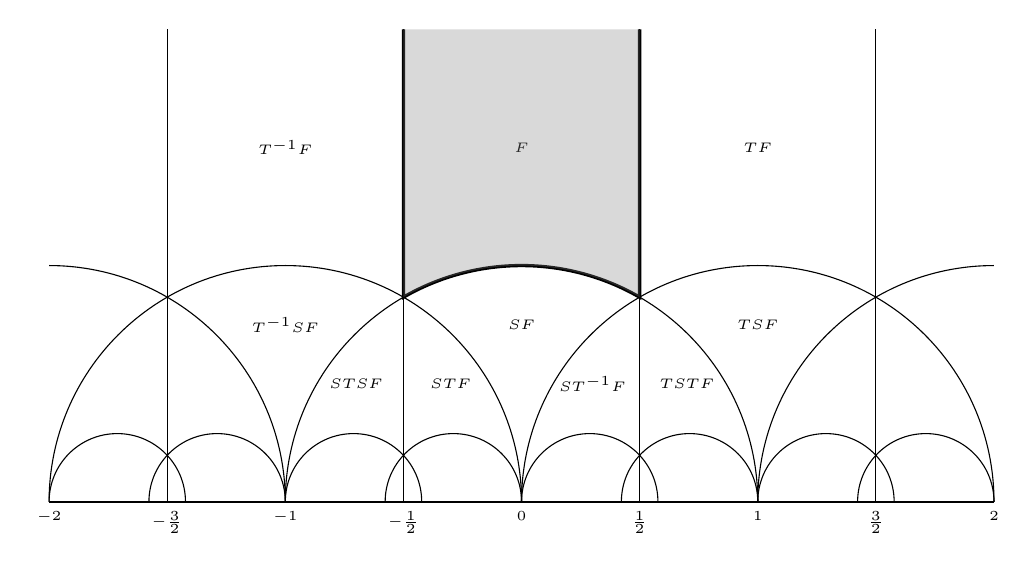
\begin{tikzpicture}[scale=3]
          \def\xmin{-2} \def\xmax{2}
          \def\ymin{0} \def\ymax{2}
          \draw[thick] (\xmin,0) -- (\xmax,0);

          \draw[very thick] (0.5,\ymax) -- (0.5,{sqrt(3)/2}) arc (60:120:1) -- (-0.5,\ymax);

          \node at (-0.5,0) [below] {\tiny{$-\frac{1}{2}$}};
          \node at (0.5,0) [below] {\tiny{$\frac{1}{2}$}};
          \node at (-1.5,0) [below] {\tiny{$-\frac{3}{2}$}};
          \node at (1.5,0) [below] {\tiny{$\frac{3}{2}$}};
          \node at (0,0) [below] {\tiny{$0$}};
          \node at (-1,0) [below] {\tiny{$-1$}};
          \node at (1,0) [below] {\tiny{$1$}};
          \node at (-2,0) [below] {\tiny{$-2$}};
          \node at (2,0) [below] {\tiny{$2$}};

          \draw[thin] (0.5,0) -- (0.5,\ymax);
          \draw[thin] (-0.5,0) -- (-0.5,\ymax);
          \draw[thin] (1.5,0) -- (1.5,\ymax);
          \draw[thin] (-1.5,0) -- (-1.5,\ymax);

          \draw (1,0) arc (0:180:1);
          \draw (-1,0) arc (0:90:1);
          \draw (2,1) arc (90:180:1);

          \draw (0,0) arc (0:180:1);
          \draw (2,0) arc (0:180:1);

          \draw (1,0) arc (0:180:{sqrt(3)/6});
          \draw ({sqrt(3)/3},0) arc (0:180:{sqrt(3)/6});

          \draw (2,0) arc (0:180:{sqrt(3)/6});
          \draw ({1+sqrt(3)/3},0) arc (0:180:{sqrt(3)/6});

          \draw (0,0) arc (0:180:{sqrt(3)/6});
          \draw ({(sqrt(3)/3)-1},0) arc (0:180:{sqrt(3)/6});

          \draw (-1,0) arc (0:180:{sqrt(3)/6});
          \draw ({(sqrt(3)/3)-2},0) arc (0:180:{sqrt(3)/6});

          \node at (0,1.5) {\tiny{$\mc{F}$}};
          \node at (-1,1.5) {\tiny{$T^{-1}\mc{F}$}};
          \node at (1,1.5) {\tiny{$T\mc{F}$}};
          \node at (0,0.75) {\tiny{$S\mc{F}$}};
          \node at (-1,0.75) {\tiny{$T^{-1}S\mc{F}$}};
          \node at (1,0.75) {\tiny{$TS\mc{F}$}};
          \node at (-0.7,0.5) {\tiny{$STS\mc{F}$}};
          \node at (-0.3,0.5) {\tiny{$ST\mc{F}$}};
          \node at (0.3,0.5) {\tiny{$ST^{-1}\mc{F}$}};
          \node at (0.7,0.5) {\tiny{$TST\mc{F}$}};

          \begin{scope}
            \path[clip] (0.5,\ymax) -- (0.5,{sqrt(3)/2}) arc (60:120:1) -- (-0.5,\ymax) -- cycle;
            \fill[gray,opacity=0.3] (-0.5,0) rectangle (0.5,\ymax);
          \end{scope}
        \end{tikzpicture}
        \caption{The standard fundamental domain for $\PSL_{2}(\Z)\backslash\H$.} \label{fig:fundamental_domain_modular_group}
      \end{figure}
      
      The shaded region in \cref{fig:fundamental_domain_modular_group} is the fundamental domain in \cref{prop:fundamental_domain_modular_group} and we call it the \textbf{standard fundamental domain}\index{standard fundamental domain}. \cref{fig:fundamental_domain_modular_group} also displays how this fundamental domain changes under the actions of the generators of $\PSL_{2}(\Z)$ as in \cref{prop:PSL_generator}. A fundamental domain for any other modular curve can be built from the standard fundamental domain as the following proposition shows (see \cite{kilford2015modular} for a proof):

      \begin{proposition}\label{prop:fundamental_domain_congruence_subgroup}
        Let $\G$ be any congruence subgroup. Then
        \[
          \mc{F}_{\G} = \bigcup_{\g \in \G\backslash\PSL_{2}(\Z)}\g\mc{F},
        \]
        is a fundamental domain for $\G\backslash\H$.
      \end{proposition}

      We might notice that $\mc{F}$ in \cref{fig:fundamental_domain_modular_group} is unbounded as it doesnt contain the point $\infty$. However, if we consider $\mc{F} \cup \{\infty\}$ then it would appear that this space is compact. The point $\infty$ is an example of a cusp and we now make this idea precise. Since any $\g \in \PSL_{2}(\Z)$ preserves $\hat{\R}$ and $\g$ has integer entries, $\g$ also preserves $\Q \cup \{\infty\}$. A \textbf{cusp}\index{cusp} of $\GH$ is an element of of $\G\backslash(\Q \cup \{\infty\})$. As $\G$ has finite index in the modular group, there can only be finitely many cusps and the number of cusps is at most the index of $\G$. In particular, the $\G$-orbit of $\infty$ is a cusp of $\GH$. We denote cusps by gothic characters $\mf{a},\mf{b},\mf{c},\ldots$ or by representatives of their equivalence classes. For example, we let $\infty$ denote the cusp $\G\infty$.

      \begin{remark}
        It turns out that the cusps can be represented as the points needed to make a fundmantal domain $\mc{F}_{\G}$ compact as a subset of $\hat{\C}$. To see this, suppose $\mf{a}$ is a limit point of $\mc{F}_{\G}$ that does not belong to $\mc{F}_{\G}$. Then $\mf{a} \in \hat{\R}$. In the case of the standard fundmantal domain $\mc{F}$, $\mf{a} = \infty$ which is a cusp. Otherwise, $\mc{F}_{\G}$ is a union of images of $\mc{F}$ by \cref{prop:fundamental_domain_congruence_subgroup} and since $\PSL_{2}(\Z)\infty = \Q \cup \{\infty\}$, we find that $\mf{a} \in \Q \cup \{\infty\}$.
      \end{remark}

      Let $\G_{\mf{a}} \le \G$ denote the stabilizer subgroup of the cusp $\mf{a}$. For the $\infty$ cusp, we can describe $\G_{\infty}$ explicitly. If $\g = \begin{psmallmatrix} a & b \\ c & d \end{psmallmatrix} \in \G$ stabilizes $\infty$, then necessarily $c = 0$ and since $\det(\g) = 1$ we must have $a = d = 1$. Therefore $\g = \begin{psmallmatrix} 1 & b \\ 0 & 1 \end{psmallmatrix}$ for some $b \in \Z$ and $\g$ acts on $\H$ by translation by $b$. Of course, not every translation is guaranteed to belong to $\G$. Letting $t$ be the smallest positive integer such that $\begin{psmallmatrix} 1 & t \\ 0 & 1 \end{psmallmatrix} \in \G$, we have $\G_{\infty} = \left\<\begin{psmallmatrix} 1 & t \\ 0 & 1 \end{psmallmatrix}\right\>$. In particular, $\G_{\infty}$ is an infinite cyclic group. We say that $\G$ is \textbf{reduced at infinity}\index{reduced at infinity} if $t = 1$ so that $\G_{\infty} = \left\<\begin{psmallmatrix} 1 & 1 \\ 0 & 1 \end{psmallmatrix}\right\>$. In particular, $\G_{1}(N)$ and $\G_{0}(N)$ are reduced at infinity.
      
      \begin{remark}
        If $\G$ is of level $N$, then $N$ is the smallest positive integer such that $\G(N) \le \G$ so that $\begin{psmallmatrix} 1 & N \\ 0 & 1 \end{psmallmatrix}$ is the minimal translation guaranteed to belong to $\G$. However, there may be smaller translations so in general $t \le N$.
      \end{remark}
      
      Actually, for any cusp $\mf{a}$, $\G_{\mf{a}}$ is also an infinite cyclic group. To see this, if $\mf{a} = \frac{a}{c}$ with $(a,c) = 1$ is a cusp of $\GH$ not equivalent to $\infty$, then there exists an $\s_{\mf{a}} \in \PSL_{2}(\Z)$ such that $\s_{\mf{a}}\infty = \mf{a}$. Indeed, there exists integers $d$ and $b$ such that $ad-bc = 1$ by B\'ezout's identity and then $\s_{\mf{a}} = \begin{psmallmatrix} a & b \\ c & d \end{psmallmatrix}$ is such a matrix. It follows that $\G_{\mf{a}} = \s_{\mf{a}}\G_{\infty}\s_{\mf{a}}^{-1}$ and since $\G_{\infty}$ is infinite cyclic so is $\G_{\mf{a}}$. We call any matrix $\s_{\mf{a}} \in \PSL_{2}(\Z)$ such that $\s_{\mf{a}}\infty = \mf{a}$ a \textbf{scaling matrix}\index{scaling matrix} for the cusp $\mf{a}$. Note that $\s_{\mf{a}}$ is determined up to composition on the right by an element of $\G_{\infty}$ or composition on the left by an element of $\G_{\mf{a}}$. Scaling matrices are useful because they allow us to transfer information at the cusp $\mf{a}$ to the cusp at $\infty$. Let $\mf{a}$ and $\mf{b}$ be cusps of $\GH$ with scaling matrices $\s_{\mf{a}}$ and $\s_{\mf{b}}$ respectively. When investigating holomorphic forms, it will be useful to have a double coset decomposition for sets of the form $\s_{\mf{a}}^{-1}\G\s_{\mf{b}}$. This is referred to as the \textbf{Bruhat decomposition}\index{Bruhat decomposition} for $\G$:

      \begin{theorem}[Bruhat decomposition]
        Let $\G$ be any congruence subgroup and let $\mf{a}$ and $\mf{b}$ be cusps of $\GH$ with scaling matrices $\s_{\mf{a}}$ and $\s_{\mf{b}}$ respectively. Then we have the disjoint decomposition
        \[
          \s_{\mf{a}}^{-1}\G\s_{\mf{b}} = \d_{\mf{a},\mf{b}}\W_{\infty}\cup\bigcup_{\substack{c \ge 1 \\ d \tmod{c}}}\W_{d/c},
        \]
        where
        \[
        \W_{\infty} = \left\{\begin{pmatrix} \ast & b \\ 0 & \ast \end{pmatrix}:\begin{pmatrix} \ast & b \\ 0 & \ast \end{pmatrix} \in \s_{\mf{a}}^{-1}\G\s_{\mf{b}}\right\},
        \]
        and
        \[
          \W_{d/c} = \G_{\infty}\w_{d/c}\G_{\infty},
        \]
        for some $\w_{d/c} = \begin{psmallmatrix} \ast & \ast \\ c & d \end{psmallmatrix} \in \s_{\mf{a}}^{-1}\G\s_{\mf{b}}$ with $c \ge 1$.
      \end{theorem}
      \begin{proof}
        We first show that $\W_{\infty}$ is nonempty if and only if $\mf{a} = \mf{b}$. Indeed, if $\w_{\infty} \in \W_{\infty}$ then $\w_{\infty} = \s_{\mf{a}}^{-1}\g\s_{\mf{b}}$ for some $\g \in \G$. Then
        \[
          \g\mf{b} = \s_{\mf{a}}\w_{\infty}\s_{\mf{b}}^{-1}\mf{b} = \s_{\mf{a}}\w_{\infty}\infty = \s_{\mf{a}}\infty = \mf{a}.
        \]
        This shows that $\mf{a} = \mf{b}$. Conversely, suppose $\mf{a} = \mf{b}$. Then $\s_{\mf{a}}^{-1}\G\s_{\mf{b}}$ contains $\s_{\mf{a}}^{-1}\G_{\mf{a}}\s_{\mf{a}} = \G_{\infty}$ so that $\W_{\infty}$ is nonempty. So $\W_{\infty}$ is nonempty if and only if $\mf{a} = \mf{b}$. In this case, for any two elements $\w_{\infty} = \s_{\mf{a}}^{-1}\g\s_{\mf{a}}$ and $\w'_{\infty} = \s_{\mf{a}}^{-1}\g'\s_{\mf{a}}$ of $\W_{\infty}$, we have
        \[
          \g'\g^{-1}\mf{a} = \s_{\mf{a}}\w'_{\infty}w_{\infty}^{-1}\s_{\mf{a}}^{-1}\mf{a} = \s_{\mf{a}}\w'_{\infty}w_{\infty}^{-1}\infty = \s_{\mf{a}}\mf{a}.
        \]
        Hence $\g'\g^{-1} \in \G_{\mf{a}}$ which implies $\w'_{\infty}w_{\infty}^{-1} = \s_{\mf{a}}^{-1}\g'\g^{-1}\s_{\mf{a}} \in \s_{\mf{a}}^{-1}\G_{\mf{a}}\s_{\mf{a}} = \G_{\infty}$. Therefore
        \[
          \W_{\infty} = \G_{\infty}w_{\infty} = w_{\infty}\G_{\infty} = \G_{\infty}w_{\infty}\G_{\infty},
        \]
        where the latter two equalities hold because $w_{\infty}$ is a translation and translations commute. Every other element of $\s_{\mf{a}}^{-1}\g\s_{\mf{b}}$ belongs to one of the double cosets $\W_{d/c}$ with $c \ge 1$ (since we are working in $\PSL_{2}(\Z)$). The relation
        \[
          \begin{pmatrix} 1 & n \\ 0 & 1 \end{pmatrix}\begin{pmatrix} \ast & \ast \\ c & d \end{pmatrix}\begin{pmatrix} 1 & m \\ 0 & 1 \end{pmatrix} = \begin{pmatrix} \ast & \ast \\ c & cm+d \end{pmatrix},
        \]
        shows that $\W_{d/c}$ is determined uniquely by $c$ and $d \tmod{c}$. This completes the proof of the theorem.
      \end{proof}

      As a first application, take $\mf{a} = \mf{b} = \infty$ and $\s_{\mf{a}} = \s_{\mf{b}} = I$. Then the Bruhat decomposition implies
      \[
        \GG \cong I\cup\bigcup_{\substack{c \ge 1 \\ d \tmod{c}}}\w_{d/c}\G_{\infty},
      \]
      since $\G_{\infty}\backslash\W_{\infty} = \G_{\infty}\backslash\G_{\infty} \cong I$. This shows that every element of $\GG$ corresponds to a unique $(c,d) \in \Z^{2}-\{\mathbf{0}\}$ with $c \ge 0$ and $d$ determined only modulo $c$ except when $c = 0$ in which case $d = 1$ (the pair $(1,0)$ corresponds to $I$). Of course, this correspondence might not be surjective since the double coset $\W_{d/c}$ may be empty if there is no $\w_{d/c} \in \s_{\mf{a}}^{-1}\G\s_{\mf{b}}$. For example, if $\G$ is of level $N$ then every $\g = \begin{psmallmatrix} a & b \\ c & d \end{psmallmatrix} \in \G$ satisfies $c \equiv 0 \tmod{N}$ so that
      \[
        \GG = I\cup\bigcup_{\substack{c \ge 1 \\ c \equiv 0 \tmod{N} \\ d \tmod{c}}}\w_{d/c}\G_{\infty}.
      \]
      However, we still may have other cosets which are empty since $\G$ being of level $N$ only guarantees that $c \equiv 0 \tmod{N}$. To figure out for what subset of pairs $(c,d)$ the correspondence is a bijection it suffices to determine the admissible $d$ not just the admissible $d \tmod {c}$. 
      
      \begin{remark}\label{rem:Bruhat_bijection}
        An exceptionally important case is for the Hecke congruence subgroups $\G_{0}(N)$ with $\mf{a} = \mf{b} = \infty$. Suppose $c \ge 1$ with $c \equiv 0 \tmod{N}$ and $d \tmod{c}$. By Bezout's identity there exists integers $a$ and $b$ with $ad-bc = 1$ so that $\g = \begin{psmallmatrix} a & b \\ c & d \end{psmallmatrix} \in \G_{0}(N)$ if and only if $(c,d) = 1$. So we must have $d \equiv 1 \tmod{c}$. Then the following correspondence implied by the Bruhat decomposition is a bijection:
        \[
          \GG = I\cup\bigcup_{\substack{c \ge 1, d \in \Z \\ c \equiv 0 \tmod{N} \\ (c,d) = 1}}\w_{d/c}\G_{\infty}.
        \]
      \end{remark}
  